\documentclass[a4paper, 11pt]{article}

\usepackage[utf8x]{inputenc}
\usepackage[T1]{fontenc}
\usepackage{ucs}
\usepackage[english]{babel}
\usepackage{mathtools, amsmath, amsfonts}
\usepackage{fancyhdr}
\usepackage[parfill]{parskip}
\usepackage{graphicx}
\usepackage{palatino,newtxmath}
\usepackage{float}
\usepackage[font={small,it}]{caption}
\usepackage{fixltx2e}
\usepackage[scaled]{helvet}
% \usepackage{fullpage}

\linespread{1.05}
\pagestyle{fancyplain}
\fancyhead{}
\fancyfoot[L]{}
\fancyfoot[C]{}
\fancyfoot[R]{\thepage}
\renewcommand{\headrulewidth}{0pt}
\renewcommand{\footrulewidth}{0pt}
\setlength{\headheight}{13.6pt}

\widowpenalty=1000
\clubpenalty=1000

\newcommand{\horrule}[1]{\rule{\linewidth}{#1}}

\title{ 
\normalfont \normalsize 
\textsc{University of Copenhagen} \\ [25pt]
\horrule{0.5pt} \\[0.4cm]
\huge PCSD: Exam \\
\horrule{2pt} \\[0.5cm]
}

\author{Jens Fredskov (chw752)}

\begin{document}
\maketitle

\newpage
\part{Exercises} % (fold)
\label{prt:exercises_}

\section{Proximity} % (fold)
\label{sec:proximity}

I assume we use a two-phase, multiway merge-sort algorithm which uses quick-sort to sort each sublist which fits in main memory (as described in \cite{chap10}). This means that $d$ will be the number of sublists we must split our data into to sort it all in main memory. Here I assume that $d$ is the combined number of sublists for $N_1$ and $N_2$.

% \paragraph{a)} % (fold)

% paragraph a_ (end)

\paragraph{b)} % (fold)

Each sublist must contain $\lfloor K_d \rfloor \vee \lfloor K_d + 1 \rfloor$ record keys where $K_d = \frac{N_1 + N_2}{d}$, as this gives the number of records per sublist. As an approximation we simply say that each sublist contains $K_d$ record keys. Of course $K_d$ might not be and integer, but if we assume so, we still get a very close approximation.

To completely fill main memory once we must transfer $\frac{M}{B} = K_B$ blocks. For the first phase of the algorithm we must fill main memory $d$ times as we have $d$ sublists. Of course we also need to transfer the sorted sublists back to disk. Thus if we assume that we sort the sublists in place (to avoid having to swap parts of the sublists back to disk) we must for phase one transfer $(2 \cdot K_B \cdot d)$ blocks of size $B$.

For the second phase we assume that $d \cdot k \le M$, meaning that we can hold one key from each sublist in memory at a time. As we now sort the sublists by transferring every nth record key and sorting these we must transfer $d$ keys (one from each sublist) $K_d$ times (the average length of the sublists). We again of course need to transfer both ways and thus we must transfer $(2 \cdot d \cdot K_d)$ record keys of size $k$.

If we assume that we only need to sort the keys, as these can be use to access the actual data, we are done after sorting the keys and thus we have an IO-cost of approximately
\[
    (2 \cdot K_B \cdot d) B + (2 \cdot d \cdot K_d) k =
    2 d (M + N_1 + N_2)
\]

% paragraph b_ (end)

% \paragraph{c)} % (fold)

% paragraph c_ (end)

% section proximity (end)

\section{Parallelism} % (fold)
\label{sec:parallelism}

\paragraph{a)} % (fold)

The first hash-function has every record of $R$ and $S$ as its domain. Potentially it has any record with the same fields as those in $R$ and $S$ as its domain, if we assume that it can be used for other records of the same type. The range of the function is $[1, k]$ as every record must map to one of the $k$ buckets corresponding to its relation.

The second hash-function has $[1, k]$ as its domain as we only need to map the buckets from before, and since every $i$th bucket must match to the same processor. The range of the function is $[1, p]$ as every bucket must map to one of the $p$ processors.
% paragraph a_ (end)

\paragraph{b)} % (fold)

Figure \ref{fig:hashjoin} explains the algorithm in general, schematically.

\begin{figure}[H]
  \centering
  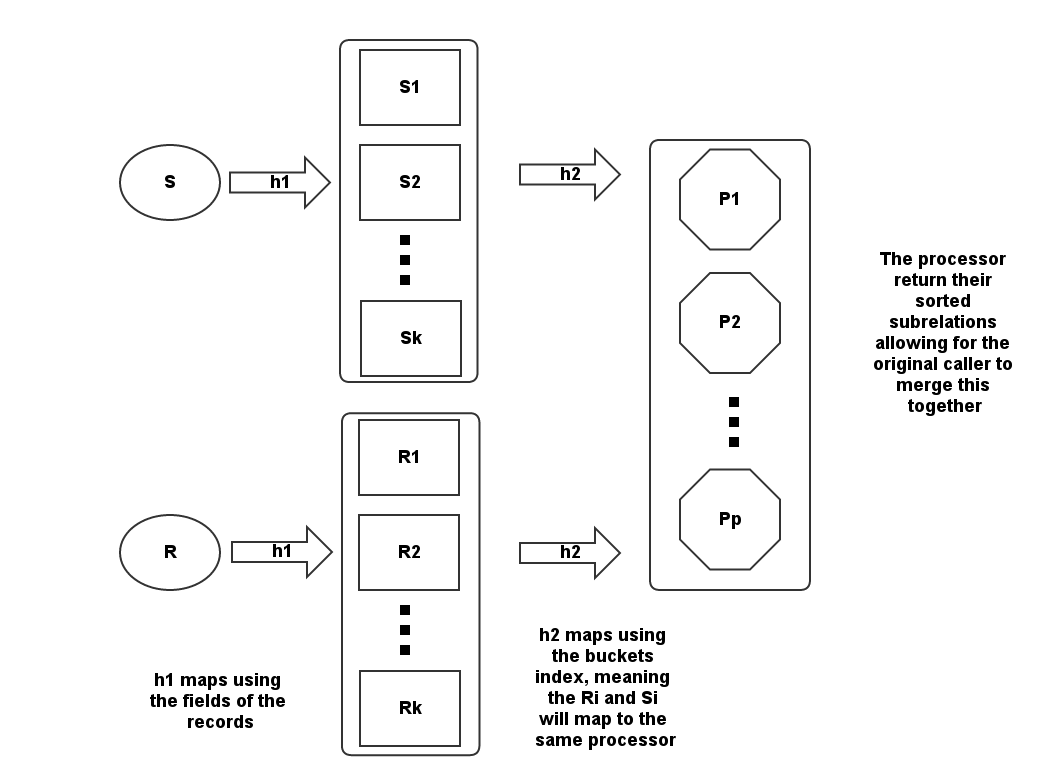
\includegraphics[width=1\textwidth]{hashjoin.png}
  \caption{A schematic explanation of the given hashjoin algorithm.}
  \label{fig:hashjoin}
\end{figure}

% paragraph b_ (end)

\paragraph{c)} % (fold)

Under the assumption of uniform hashing we have that the average size of a bucket $R_i = \frac{B(R)}{k}$ and $S_i = \frac{B(S)}{k}$. Furthermore each processor will have an average of $\frac{k}{p}$ buckets from each relation mapped to it, which means that a one-pass should be enough as each processor can hold $O(k)$ pages. If we assume that the processors receive their buckets and do not themselves partition the relations, they must spend
\[
 \frac{k}{p} (\frac{B(R) + B(S)}{k})   
\]
to write their buckets to disk, the same amount to do the one-pass join, and finally the same amount when reading from disk and sending their results back. This means that every processor performs
\[
    3 \frac{k}{p} \left(\frac{B(R) + B(S)}{k}\right) = 3 \frac{B(R) + B(S)}{p}
\]

% paragraph c_ (end)

% \paragraph{d)} % (fold)

% paragraph d_ (end)

% section parallelism (end)

% part exercises_ (end)

\newpage
\part{Programming} % (fold)
\label{prt:programming_}

\section{High-Level Design Decisions and Modularity} % (fold)
\label{sec:high_level_design_decisions_and_modularity}

\paragraph{Question 1} % (fold)
\label{par:question_1}

Using the proxies (\texttt{OrderManagerHTTPProxy} and \texttt{Item\-SupplierHTTPProxy}), which work as RPC stubs that communicate with the servers, \textit{exactly-once} semantics are effectively implemented between the clients, and OrderManagers/ItemSuppliers. Using just the proxies we have \textit{at-most-once} semantics, however as we also log every action we could at a later point implement recovery, meaning that we would be able to recover from a failure, giving us the \textit{exactly-once} semantics. Between the OrderManager and the ItemSupplier the \textit{at-most-once} semantics are implemented. Each step in the OrderManager runs in its own task (to make the workflow asynchronous) these try to contact the respective ItemSuppliers they need over HTTP. At the moment if a request times out or if the supplier is unavailable the request will fail, and the status of the step is set to failed meaning that is what a caller will see when trying asking for the status. Using the logging we could either retry failed steps at a later time, or we could change the tasks slightly so they retry if they get exceptions about timeouts or servers being unavailable, giving \textit{exactly-once} semantics.

The asynchronous execution of workflows in the OrderManager has been implemented in the following way. The class \texttt{CertainOrderManager} utilizes an executor with a thread pool. Whenever a workflow is registered, each step is checked to make sure that the OrderManager knows the supplier and if so the steps a wrapped in a request object. The new list of request objects are given to the executor which submits submits a callable \texttt{OrderStepTask} for each request to the thread pool and finally returns a list of future result objects to the OrderManager. These are saved in a map under the workflow id, and the id is then returned to the caller. If a caller asks for a registered workflow id the OrderManager tries to get the result of each task. If a task is done its result is added to the list of statuses (either successful or failed), otherwise a registered status is added to the list.

Upon failure in either a OrderManager or ItemSupplier (\texttt{CertainOrder\-Manager} and \texttt{CertainItemSupplier}) an exception is thrown as dictated by the interfaces they implement. In the server handlers (\texttt{Order\-ManagerHTTPMessageHandler} and \texttt{ItemSupplierHTTPMesageHandler}) these exceptions are caught, as to avoid the entire server from crashing on a failure. The message handlers instead set the exception in the response it needs to send, and then sends this response back. In the proxies (\texttt{OrderManagerHTTPProxy} and \texttt{ItemSupplierHTTPProxy}) these exception are unpacked from the response and thrown again, as the proxies also implement the interfaces. The OrderManager when it processes steps however does not throw exceptions if a step receives such a response from an ItemSupplier. Instead the task responsible for the given step simple sets a success flag in its response to false. In this way when a caller asks for the status of the workflow they see a failed status for that step. This stops the task or potentially the entire OrderManager from crashing.

% paragraph question_1 (end)

% section high_level_design_decisions_and_modularity (end)

\section{Atomicity and Fault-Tolerance} % (fold)
\label{sec:atomicity_and_fault_tolerance}

\paragraph{Question 2} % (fold)
\label{par:question_2}

To ensure serializability at each ItemSupplier a read/write lock is utilized. Whenever the ItemSupplier tries to execute a step it first takes a write lock, as this action includes both reading the items of the supplier and later on writing the new updated quantities. However when the ItemSupplier tries to get the number of orders for a set of items it need only take a read lock. This allows several clients to get order quantities without blocking each other. However when someone wishes to update the orders they must have exclusive access. This approach makes sure that no one get dirty reads.

As there is only one lock per ItemSupplier, the method utilized is not only equivalent to, but is, strict two-phase locking. The lock is always taken before the part of the method which interacts with the ItemSuppliers map of items. Furthermore, it is released only when the method is done using the map. Finally when first the lock is released the lock is not reacquired in the method, thus in this way we are actually using a strict two-phase locking approach.

If we consider the workload an ItemSupplier is exposed to it would seem realistic that it would receive more requests to execute steps than it would to check for orders, as each workflow can consist of many steps, of which several may be directed to the same ItemSupplier, and that several OrderManagers may request execution of steps. Considering this, it would have been nice to be able to allow either to process steps concurrently or to just check and accept them, and then process them at a later time (This however is alleviated by OrderManagers as they themselves process steps asynchronously). Thus a mechanism which could have provided better performance than the simple read/write lock would be a multi-granularity lock. Using this locking scheme we could have asked asked to read or write only the item ids we needed per transaction. This would potentially allow several writes running concurrently, as long as they write to different item ids.

The read/write lock however is much simpler to implement (and thus get right) and is in this case most probably better than both optimistic approach and queuing operations. The latter is obviously worse, as it disallows even concurrent reads of orders, whereas the optimistic approach probably performs worse as it risks often having to do rollbacks on reads, if we assume many more executions of steps than reads of orders. Furthermore the optimistic approach, and the rollback feature it implies, is a lot harder to correctly implement.

% paragraph question_2 (end)

\paragraph{Question 3} % (fold)
\label{par:question_3}
The OrderManager logs every workflow it registers, with a supplier id, all its order steps and their respective item ids and quantities. Furthermore every time a task running one of the steps completes, meaning that it has received an answer from the supplier, it adds an entry to the log with the steps workflow id, which step in the workflow it was, and whether the step succeeded or failed (resulted in an error). To recover from a failure in the OrderManager we could do the following. First we read in the entire log and identify all workflows which are completely registered, meaning that it should begin with \texttt{WORKFLOW BEGIN id} and end with either \texttt{WORKFLOW END} or \texttt{WORKFLOW CANCELLED}. Canceled workflows can be thrown away. There can at maximum be one not ended workflow as methods in the OrderManager are synchronized. If a workflow has not been ended its steps was never submitted and thus they must all be submitted to their suppliers (using the executor). If a workflow was properly ended we must scour the log for every \texttt{SUCCSTEP} and \texttt{FAILSTEP} entry belonging to that workflow. All steps which were not registered should be resubmitted to their suppliers.

%TODO: something about how we might submit in a task and crash while the itemsupplier actually correctly does the step. Is it better to say when we start a submission and then if we fail midways throw it away just to avoid duplicating steps?

The ItemSupplier logs every step that it starts executing and whether the step was successful or failed. To recover from a failure in the ItemSupplier we could do the following. First we read the entire log. Every successful step we replay and every canceled step we throw away.
% paragraph question_3 (end)

% section atomicity_and_fault_tolerance (end)

\pagebreak
\section{Testing} % (fold)
\label{sec:testing}

\paragraph{Question 4} % (fold)
\label{par:question_4}

To test the OrderManager the following strategy is used. Random steps are generated and combined into workflows. After a workflow is registered we enter a \textit{do-while} loop where we ask for the status of the workflow. As long as parts of the workflow are still only registered and not completed (either successfully or failed) we ask again. In this way we can query for the status of the workflow until the entire flow is complete. In the tests where we expect everything to work (that is where quantities are not negative, the item supplier exists and has all the item ids we ask to increase) no step must have the failed status. In the tests where something should go wrong we let all steps be failing steps, and then no step should have the successful status.

To test that the methods of the ItemSupplier are atomic the following strategy is used. Two threads are created that both communicate with the same ItemSupplier. One constantly submits steps where all items have their quantities increased with one. The other thread constantly ask for all items quantities and check their the amount they have changed from the first request it did. If the methods are indeed atomic, it is expected that all items have increased with the same amount, since the last read. If they however are not atomic we would expect the thread which checks to get a dirty read at some point, and see different increments in the items quantities.

To test error conditions of the components the following strategy was used. For the OrderManager, and the ItemSupplier, tests with clients are run, where wrong item ids, quantities and supplier ids are given. For the ItemSupplier all errors should result in an exception being thrown and this is thus the expected outcome of the these tests. For the OrderManager a wrong supplier id or workflow id will result in an exception, whereas wrong item ids and quantities will result in a failed status of that step. Thus the latter does not have an exception as their expected outcome, but instead that their steps fail. Finally tests are done where both ends of the supply chain are checked.That is when an OrderManager supplies wrong item ids or negative quantities, it receives a failed status of that step, and the ItemSupplier does not increase the quantities.

All tests finishes successfully.

% paragraph question_4 (end)

% section testing (end)

\pagebreak
\section{Experiments} % (fold)
\label{sec:experiments}

\paragraph{Question 5} % (fold)
\label{par:question_5}

The experiment in general utilizes the same approach as was used in assignment 3 of the course. That is we run a thread pool with more and more threads all running a worker with has some task. The tasks either run an OrderManager interaction or they run a local ItemSupplier client interaction. Which they choose is random but controlled by a percentage/ratio in the configuration of the worker. Each worker does a series of warm up runs first and then afterwards do their actual runs which they measure. The measures from all workers in a thread pool are aggregated and computed on, to get the aggregate throughput, average latency, successful interactions and ratio of OrderManager interactions over all its runs. The two last are used to check that the workload mix is as expected and that we do not have to many failed interactions. This is done for the same number of workers a number of times to average over the values.

Specifically the workload mix used in the experiment is that 80\% of the interactions should be OrderManager interactions, as it is expected that it will mostly be the OrderManagers who order more of items and then occasionally will a client check what is ordered. Every OrderStep contains 3 steps, which is arbitrarily chosen and each step can order up to 1000 of each item, as we might expect wholesalers to order large quantities. Each ItemSupplier interaction can ask for a random number of its ids. Each worker does 10 warm up runs and then 30 actual runs. The number of workers run from 2 to 14 increasing with 2 every step. For each step 3 runs are done, over which the results are averaged.

Preferably the number of runs should have been even higher, but on a single computer this gives some problems with exceptions from Jetty because it cannot shutdown threads in its internal thread pool and thus use up all available connections. Thus the number of runs was downscaled to successfully run the experiment.

The experiment was run on a single computer with the following specifications:
\begin{table}[H]
\centering
\begin{tabular}{rl}
CPU: & Intel Core i7 @ 2.80 GHz \\
RAM: & 8GB \\
Operating System: & Arch Linux \\
Hard drive: & ATA Samsung SSD 830 \\
\end{tabular}
\end{table}
As the setup contains eight logical cores we might expect to see the throughput rise up until somewhere just around eight workers which would be the maximal number of workers that could run at the same time.

After running the experiment the data outputted was as seen in Table \ref{tab:data}. Using these and averaging over each number of workers, the aggregated throughput and average latency have been plotted in Figure \ref{fig:throughput} and Figure \ref{fig:latency}.

When looking at the graphs we see the throughput rise until it reaches eight concurrent workers, then fall again and on the last rise. In the same way the latency starts rising at eight workers, but drops again at 14. the fact that we see a change at eight workers might be attributed to the setup which has eight cores. However many other factors might play in. Especially the fact that Jetty seems to be having problems with shutting downs threads in its internal thread pool when it reaches just around eight to 10 workers. Another issue is the fact that the last data point shows a high throughput, this might indicate that the setup was disturbed at 10 and 12 workers (e.g. by the operating system working behind the scenes). Thus the results of the experiment are somewhat unclear, but it seems that the ItemSupplier scales well/linear up until around eight concurrent workers (remember that they all submit more than one OrderStep, meaning that the ItemSupplier handles more than eight requests at that point).

\begin{table}[H]
\centering
\footnotesize
\begin{tabular}{ccccc}
Workers & Throughput (succXact/s) & latency (s) & SuccRatio & orderManagerXactRatio \\ \hline
2  & 28.7257  & 2.0949 & 1 & 0.85 \\
2  & 31.4281  & 1.9123 & 1 & 0.8  \\
2  & 31.6338  & 1.898  & 1 & 0.82 \\
4  & 59.6614  & 2.014  & 1 & 0.83 \\
4  & 65.9829  & 1.8226 & 1 & 0.79 \\
4  & 61.81    & 1.9486 & 1 & 0.85 \\
6  & 93.7409  & 1.9417 & 1 & 0.81 \\
6  & 92.1887  & 1.9548 & 1 & 0.78 \\
6  & 90.9345  & 1.9981 & 1 & 0.77 \\
8  & 102.2635 & 2.3603 & 1 & 0.78 \\
8  & 88.3375  & 2.7279 & 1 & 0.8  \\
8  & 90.8956  & 2.6466 & 1 & 0.8  \\
10 & 84.6169  & 3.5499 & 1 & 0.78 \\
10 & 72.1851  & 4.1574 & 1 & 0.84 \\
10 & 66.6472  & 4.5105 & 1 & 0.81 \\
12 & 57.1896  & 6.2983 & 1 & 0.8  \\
12 & 49.7696  & 7.2373 & 1 & 0.81 \\
12 & 69.5267  & 5.1944 & 1 & 0.8  \\
14 & 114.0111 & 3.6961 & 1 & 0.8  \\
14 & 108.7776 & 3.8741 & 1 & 0.82 \\
14 & 108.8745 & 3.8776 & 1 & 0.81 \\
\end{tabular}
\caption{The collected data from the experiment.}
\label{tab:data}
\end{table}

\begin{figure}[H]
  \centering
  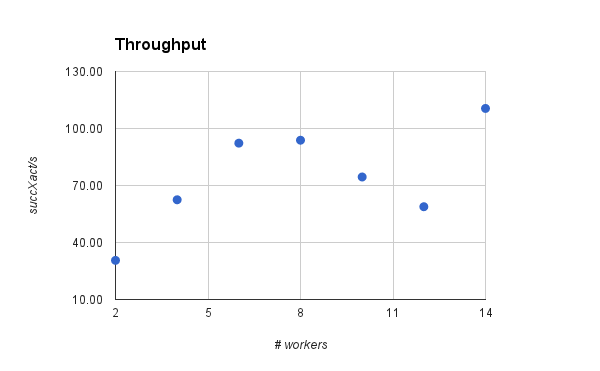
\includegraphics[width=1\textwidth]{chart_1.png}
  \caption{The aggregated throughput when running a given number of workers.}
  \label{fig:throughput}
\end{figure}

\begin{figure}[H]
  \centering
  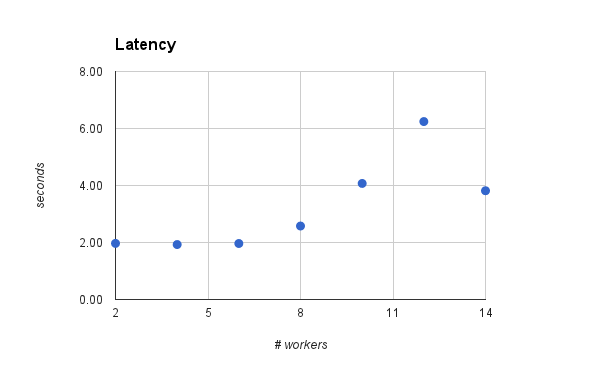
\includegraphics[width=1\textwidth]{chart_2.png}
  \caption{The average latency measured when running a given number of workers.}
  \label{fig:latency}
\end{figure}

% paragraph question_5 (end)

% section experiments (end)

% part programming_ (end)

\begin{thebibliography}{9}

\bibitem{chap10}
    H. Garcia-Molina, J. D. Ullman, J. Widom.
    Database Systems: The Complete Book,
    Chapter 11.4, pp. 525–533 (9 of 1119).
    Prentice Hall, 2002.
    ISBN: 0-13-031995-3
\end{thebibliography}

% \bibitem{chap11}
%     H. Garcia-Molina, J. D. Ullman, J. Widom.
%     Database Systems: The Complete Book.
%     Chapter 15, pp. 713–774 (62 of 1119).
%     Prentice Hall, 2002.
%     ISBN: 0-13-031995-3
\end{document}